%%%%%%%%%%%%%%%%%%%%%%%%%%%%%%%%%%%%%%%%%12pt: grandezza carattere
                                        %a4paper: formato a4
                                        %openright: apre i capitoli a destra
                                        %twoside: serve per fare un
                                        %   documento fronteretro
                                        %report: stile tesi (oppure book)
\documentclass[12pt,a4paper,openright, oneside]{report}
%
%%%%%%%%%%%%%%%%%%%%%%%%%%%%%%%%%%%%%%%%%libreria per scrivere in italiano
\usepackage[italian]{babel}
%
%%%%%%%%%%%%%%%%%%%%%%%%%%%%%%%%%%%%%%%%%libreria per accettare i caratteri
                                        %   digitati da tastiera come è à
                                        %   si può usare anche
                                        %   \usepackage[T1]{fontenc}
                                        %   però con questa libreria
                                        %   il tempo di compilazione
                                        %   aumenta

\usepackage[T1]{fontenc}
\usepackage[utf8]{inputenc}
%
%%%%%%%%%%%%%%%%%%%%%%%%%%%%%%%%%%%%%%%%%libreria per impostare il documento
\usepackage{fancyhdr}
%
%%%%%%%%%%%%%%%%%%%%%%%%%%%%%%%%%%%%%%%%%libreria per avere l'indentazione
%%%%%%%%%%%%%%%%%%%%%%%%%%%%%%%%%%%%%%%%%   all'inizio dei capitoli, ...
\usepackage{indentfirst}
%
%%%%%%%%%libreria per mostrare le etichette
%\usepackage{showkeys}
%
%%%%%%%%%%%%%%%%%%%%%%%%%%%%%%%%%%%%%%%%%libreria per inserire grafici
\usepackage{graphicx}
\usepackage{float}
%
%%%%%%%%%%%%%%%%%%%%%%%%%%%%%%%%%%%%%%%%%libreria per utilizzare font
                                        %   particolari ad esempio
                                        %   \textsc{}
\usepackage{newlfont}
%
%%%%%%%%%%%%%%%%%%%%%%%%%%%%%%%%%%%%%%%%%librerie matematiche
\usepackage{amssymb}
\usepackage{amsmath}
\usepackage{latexsym}
\usepackage{amsthm}

\usepackage{listings}
\usepackage{parcolumns}
\input{solidity-highlighting.tex}	
%
\oddsidemargin=30pt \evensidemargin=20pt%impostano i margini
\hyphenation{sil-la-ba-zio-ne pa-ren-te-si}%serve per la sillabazione: tra parentesi 
					   %vanno inserite come nell'esempio le parole 
%					   %che latex non riesce a tagliare nel modo giusto andando a capo.

%
%%%%%%%%%%%%%%%%%%%%%%%%%%%%%%%%%%%%%%%%%comandi per l'impostazione
                                        %   della pagina, vedi il manuale
                                        %   della libreria fancyhdr
                                        %   per ulteriori delucidazioni
\pagestyle{fancy}\addtolength{\headwidth}{20pt}
\renewcommand{\chaptermark}[1]{\markboth{\thechapter.\ #1}{}}
\renewcommand{\sectionmark}[1]{\markright{\thesection \ #1}{}}
\rhead[\fancyplain{}{\bfseries\leftmark}]{\fancyplain{}{\bfseries\thepage}}
\cfoot{}
%%%%%%%%%%%%%%%%%%%%%%%%%%%%%%%%%%%%%%%%%
\linespread{1.3}                        %comando per impostare l'interlinea
%%%%%%%%%%%%%%%%%%%%%%%%%%%%%%%%%%%%%%%%%definisce nuovi comandi
%
\begin{document}
\begin{titlepage}                       %crea un ambiente libero da vincoli
                
%%%%%%%%%%%%%%%%%%%%%%%%%%%%%%%%%%%%%%%%
\clearpage{\pagestyle{empty}\cleardoublepage}%non numera l'ultima pagina sinistra
\end{titlepage}
\pagenumbering{roman}                   %serve per mettere i numeri romani

\chapter*{Introduzione}                 %crea l'introduzione (un capitolo
                                       %   non numerato)
%%%%%%%%%%%%%%%%%%%%%%%%%%%%%%%%%%%%%%%%%imposta l'intestazione di pagina
\rhead[\fancyplain{}{\bfseries
INTRODUZIONE}]{\fancyplain{}{\bfseries\thepage}}
\lhead[\fancyplain{}{\bfseries\thepage}]{\fancyplain{}{\bfseries
INTRODUZIONE}}
%%%%%%%%%%%%%%%%%%%%%%%%%%%%%%%%%%%%%%%%%aggiunge la voce Introduzione
                                        %   nell'indice
\addcontentsline{toc}{chapter}{Introduzione}
Le security token offerings, abbreviate in STO, sono un fenomeno recente che si è diffuso a partire dalla seconda metà del 2017 mantenendo inizialmente la connotazione di initial coin offerings debolmente regolamentate e solo più tardi differenziate nella loro connotazione attuale di token che dal punto di vista giuridico tendono a configurarsi come securities, al pari di altri strumenti finanziari.  

Lo scopo di questo lavoro di tesi è stato approfondire la comprensione di questo fenomeno in particolare analizzandone le caratteristiche, le cause e metodologie con le quali queste STO vengono realizzate.

In primo luogo, si definiranno le caratteristiche delle initial coin offerings e successivamente verranno individuati i criteri per identificare correttamente la differenza tra queste e le security token offerings. Una volta posti questi criteri si procederà ad analizzare i dati delle security token offerings individuate al fine di poter descrivere le metriche di questo fenomeno. Una volta valutata la rilevanza delle security token offering e le prospettive di crescita e diffusione verranno analizzate e comparate le principali implementazioni di questo modello.  



%%%%%%%%%%%%%%%%%%%%%%%%%%%%%%%%%%%%%%%%%non numera l'ultima pagina sinistra
\clearpage{\pagestyle{empty}\cleardoublepage} 

\tableofcontents                        %crea l'indice
%%%%%%%%%%%%%%%%%%%%%%%%%%%%%%%%%%%%%%%%%imposta l'intestazione di pagina
\rhead[\fancyplain{}{\bfseries\leftmark}]{\fancyplain{}{\bfseries\thepage}}
\lhead[\fancyplain{}{\bfseries\thepage}]{\fancyplain{}{\bfseries INDICE}}
%%%%%%%%%%%%%%%%%%%%%%%%%%%%%%%%%%%%%%%%%non numera l'ultima pagina sinistra
\clearpage{\pagestyle{empty}\cleardoublepage}
\listoffigures                          %crea l'elenco delle figure
%%%%%%%%%%%%%%%%%%%%%%%%%%%%%%%%%%%%%%%%%non numera l'ultima pagina sinistra
\clearpage{\pagestyle{empty}\cleardoublepage}
\listoftables                           %crea l'elenco delle tabelle
%%%%%%%%%%%%%%%%%%%%%%%%%%%%%%%%%%%%%%%%%non numera l'ultima pagina sinistra


\clearpage{\pagestyle{empty}\cleardoublepage}

\chapter{Differenze tra Initial Coin Offering e Security Token Offering}                %crea il capitolo
%%%%%%%%%%%%%%%%%%%%%%%%%%%%%%%%%%%%%%%%%imposta l'intestazione di pagina
\lhead[\fancyplain{}{\bfseries\thepage}]{\fancyplain{}{\bfseries\rightmark}}
\pagenumbering{arabic}
%mette i numeri arabi


\section{Breve storia delle monete elettroniche e delle cryptocurrency}

Sebbene le valute digitali abbiano raggiunto un nuovo livello di rilievo nel mondo solo negli ultimi anni, è importante ricordare che la monete elletroniche hanno una storia che risale a decenni fa. Il white paper “Bitcoin: A Peer-to-Peer Electronic Cash System”, pubblicato nel 2008 da un autore anonimo o da un gruppo di persone sotto lo pseudonimo di Satoshi Nakamoto, per quanto risulti innovativo e a posteriori anche rivoluzionario, si basa su tecnologie preesistenti e ben affermate tra le quali ad esempio le reti P2P, un fenomeno che ha radici nelle prime fasi della storia di Internet e reso popolare da Napster. Non sono solo le reti distribuite ad essere una fondazione per Bitcoin; nel white paper Nakamoto si avvale infatti di altri lavori precedenti che risultano fondamentali al funzionamento della rete. Tra questi possiamo citare il lavoro di tesi pubblicato da Ralph Merkle nei primi anni ’70  riguardo alla comunicazione sicura attraverso canali insicuri e gli sviluppi apportati da Diffie e Hellman. Inoltre, è proprio a Merkle che dobbiamo l’invenzione dei Merkle Tree usati in Bitcoin poiché forniscono un metodo per firmare digitalmente messaggi contenuti in grandi strutture dati. I merklee tree verrano successivamente ripresi da Bayer, Haber e Stornetta per la realizzazione efficiente di una catena di blocchi firmata crittograficamente.


Altri lavori più recenti risultano essere punti chiave per lo sviluppo della rete Bitcoin ed in generale dei sistemi di pagamento elettronici.


Nel 1983 in “Blind Signatures for Untraceable Payments” e nei sui lavori successivi, Chaum introduce l’idea di un sistema di pagamento elettronico anonimo basato sulla tecnologia di Blind Signature, sistema che verrà poi implementato dallo stesso autore con ECash™ nel 1994. Come osserva Schoenmakers nonostante le istituzioni finanziare già utilizzassero dietro le quinte sistemi elettronici per processare transazioni l’apertura al pubblico dei sistemi di pagamento elettronici introduce la necessità di un sistema di pagamento elettronico che possa essere utilizzato in una rete ad accesso pubblico, particolarmente in riferimento alla rete Internet. Nel 1998 DigiCash fallisce, principalmente a causa della forte competizione posta in atto dal sistema di pagamento tramite carta di credito. Nel particolare secondo Chaum la compagnia ha sofferto di un chicken-and-egg problem: fu difficile convincere abbastanza venditori  ad adottare il sistema per  poter acquisire clienti e vice versa. (Lo stesso destino spetta ad altre forme di pagamento elettronico dello stesso periodo tra le quali possono essere citate CyberCoin, Virtual PIN. ) 


Sebbene infruttuosa, l’esperienza di Chaum rappresenta il primo esempio di un sistema di pagamento elettronico anonimo e risulta pioneristico sia nei problemi che vengono presentati come nelle soluzioni proposte a quest’ultimi, come avviene nel caso del problema di double spending. 


Altri sistemi di moneta digitale si sono susseguiti negli anni, tra i più rilevanti possiamo citare e-gold, Liberty Reserve e PayPal: I primi due non più attivi, entrambi per controversie legali, mentre l’ultimo ancora attivo. Questa lista non ha scopo di essere esauriente, per un approfondimento si rimanda alla letteratura sull’argomento.
Un altro tassello fondamentale nello sviluppo delle monete elettroniche è l’introduzione nel 1997 di hashcash da parte di Adam Back che indipendentemente descrive un sistema simile a quanto proposto da Cynthia Dwork,  Moni Naor e Eli Ponyatovski nel 1992 in “Pricing via Processing or Combatting Junk Mail”. Entrambe le proposte prevedono l’utilizzo di quella che nel 1999 viene formalizzata da  Markus Jakobsson e Ari Juels come “proof of work” per arginare il fenomeno dello spam. Appena un anno prima, nel 1998, Wei Dai introduce B-money, un sistema basato su hashcash che comprendeva varie feature oggi comuni alla maggior parte delle cryptocurrencies. B-money tuttavia non fu mai lanciato e rimase solo una proposta ma il lavoro di Dai non fu vano; dieci anni dopo, all'inizio dello sviluppo di Bitcoin, Dai fu il primo ad essere contattato da Nakamoto. A lui seguirono altri sviluppatori tra i quali Nick Szabo, creatore di bitgold, e Hal Finney, che introdusse l'idea di "reusable PoW". 

Nel 1998 infatti, Nick Szabo creò bitgold, un meccanismo per una digital currency decentralizzata e sicura che implementava già alcune idee alla base degli smart contracts. Le teorie di Szabo riguardo riguardo gli accordi auto-attuanti furono formulato all'incirca durante lo stesso periodo in cui Ian Grigg introdusse l'idea dei Ricardian Contracts, un metodo per registrare un documento come un contratto legale e collegarlo in modo sicuro ad altri sistemi. Bitgold, come B-money, non fu mai implementato.
 
 Hal Finney nel 2004 introduce la prima reusable PoW (RPoW), ancor prima della nascita di Bitcoin. Più tardi, nel 2009, Finney riceverà la prima transazione della rete Bitcoin, da parte di Nakamoto stesso. 

La pubblicazione del white paper di Btcoin avviene finalmente nel 2008, poco dopo il clou della crisi finanziaria e del collasso di Lehman Brothers. L'obbiettivo a cui Bitcoin mira è fornire una valuta digitale P2P che non necessiti della presenza di banche ed altri intermediari.  La prima implementazione di bitcoin fu opera di Nakamoto ma successivamente la direzione dei lavori passò gradualmente ad un gruppo di primi utenti e sviluppatori. 

E' interessante notare come nel suo whitepaper Nakamoto non si riferisca a "blockchain" ma solo a "chain of blocks". Il termine "blockchain" infatti si diffonde successivamente durante lo sviluppo di protocolli alternativi a bitcoin. 



\begin{figure}[H]
  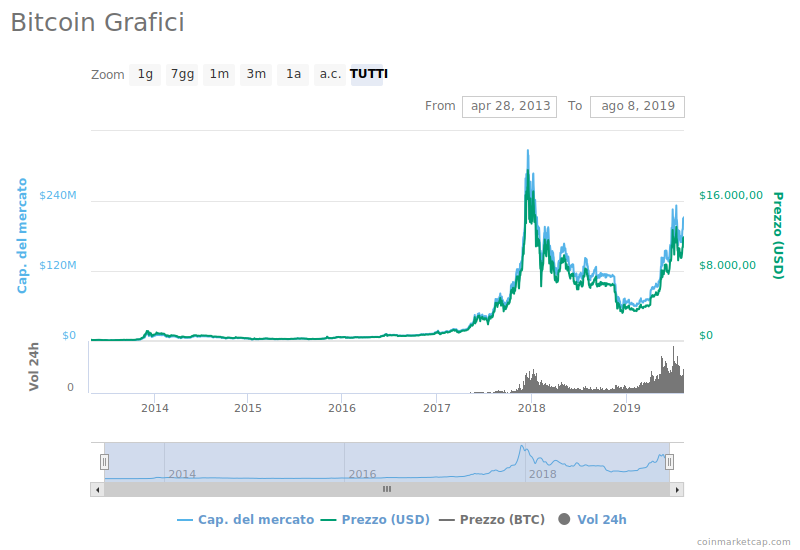
\includegraphics[width=\linewidth]{chartbitcoin.png}
  \caption{Bitcoin price chart}
  \label{fig:chartbitcoin}
\end{figure}


Ethereum viene descritto da Buterin in 

\section{Classificazione dei token nelle token sales}

\subsection{Il modello delle initial coin offering}
\subsection{Il modello delle security token offering}


\chapter{Analisi delle Security Token Offering}
++INCLUDERE DATI SEPARATI PER FONTE DEI DATI (POLYMATH, ALTRI ISSUANCE PLATFOARM, SITI AGGREGATORI)
\section{Analisi dei dati}

\section{Tendenze e previsioni}

\clearpage{\pagestyle{empty}\cleardoublepage}

\chapter{Confronto tra le implementazioni}
\section{Implementazione con token ERC-20}
\subsection{ERC-20 proprietary extension}
\section{Implementazione con token ERC-1400}
\subsection{ERC-1410: Partially Fungible Token Standard}
https://github.com/ethereum/EIPs/issues/1410
\subsection{ERC-1594: Core Security Token Standard}
https://github.com/ethereum/EIPs/issues/1594
\subsection{ERC-1643: Document Management Standard}
https://github.com/ethereum/EIPs/issues/1643
\subsection{ERC-1644: Controller Token Operation Standard}
https://github.com/ethereum/EIPs/issues/1644
\subsection{ERC-2258: Custodial Ownership Standard}
https://github.com/ethereum/EIPs/issues/2258
\section{Implementazione con }
\section{Comparazione delle implementazioni}


\input{4capitolo.tex}

\chapter{Sviluppi futuri}
https://hackernoon.com/a-comprehensive-guide-to-the-next-generation-of-crypto-funding-v-ico-ieo-daico-eto-sto-939909782da6

%%%%%%%%%%%%%%%%%%%%%%%%%%%%%%%%%%%%%%%%%per fare le conclusioni
\chapter*{Conclusioni}
%%%%%%%%%%%%%%%%%%%%%%%%%%%%%%%%%%%%%%%%%imposta l'intestazione di pagina
\rhead[\fancyplain{}{\bfseries
CONCLUSIONI}]{\fancyplain{}{\bfseries\thepage}}
\lhead[\fancyplain{}{\bfseries\thepage}]{\fancyplain{}{\bfseries
CONCLUSIONI}}
%%%%%%%%%%%%%%%%%%%%%%%%%%%%%%%%%%%%%%%%%aggiunge la voce Conclusioni
                                        %   nell'indice
\addcontentsline{toc}{chapter}{Conclusioni} Queste sono le
conclusioni.\\
In queste conclusioni voglio fare un riferimento alla
bibliografia: questo \`e il mio riferimento \cite{K3,K4}.

%%%%%%%%%%%%%%%%%%%%%%%%%%%%%%%%%%%%%%%%%imposta l'intestazione di pagina
\renewcommand{\chaptermark}[1]{\markright{\thechapter \ #1}{}}
\lhead[\fancyplain{}{\bfseries\thepage}]{\fancyplain{}{\bfseries\rightmark}}
\appendix                               %imposta le appendici
\chapter{ERC-20 Interface Implementation}               %crea l'appendice
\label{appendix:ERC-20Interface}
\lstinputlisting[language=Solidity,caption=OpenZeppelin ERC-20 Inferface Implementation,frame=tlrb]{IERC20.sol}

\lstinputlisting[language=Solidity,caption=ConsenSys ERC-20 Inferface Implementation,frame=tlrb]{EIP20Interface.sol}
%%%%%%%%%%%%%%%%%%%%%%%%%%%%%%%%%%%%%%%%%imposta l'intestazione di pagina
\rhead[\fancyplain{}{\bfseries \thechapter \:ERC-20 Interface Implementation}]
{\fancyplain{}{\bfseries\thepage}}

\chapter{Seconda Appendice}             %crea l'appendice
%%%%%%%%%%%%%%%%%%%%%%%%%%%%%%%%%%%%%%%%%imposta l'intestazione di pagina
Testo
\rhead[\fancyplain{}{\bfseries \thechapter \:Seconda Appendice}]
{\fancyplain{}{\bfseries\thepage}}

\begin{thebibliography}{90}             %crea l'ambiente bibliografia
\rhead[\fancyplain{}{\bfseries \leftmark}]{\fancyplain{}{\bfseries
\thepage}}
%%%%%%%%%%%%%%%%%%%%%%%%%%%%%%%%%%%%%%%%%aggiunge la voce Bibliografia
                                        %   nell'indice
\addcontentsline{toc}{chapter}{Bibliografia}
%%%%%%%%%%%%%%%%%%%%%%%%%%%%%%%%%%%%%%%%%provare anche questo comando:
%%%%%%%%%%%\addcontentsline{toc}{chapter}{\numberline{}{Bibliografia}}
\bibitem{K1} S. Nakamoto, “Bitcoin: A Peer-to-Peer Electronic Cash System,” p. 9.
\bibitem{K2} Merkle, R. C. (1978). Secure communications over insecure channels. Communications of the ACM, 21(4), 294-299.
\bibitem{K3} Diffie, W., and Hellman, M. New directions in cryptography. IEEE Trans. on Inform. IT-22, 6 (Nov. 1976), 644-654.
\bibitem{K4} Merkle, R. C. (1987, August). A digital signature based on a conventional encryption function. In Conference on the theory and application of cryptographic techniques (pp. 369-378). Springer, Berlin, Heidelberg.
\bibitem{K5} Bayer, D., Haber, S., \& Stornetta, W. S. (1993). Improving the efficiency and reliability of digital time-stamping. In Sequences Ii (pp. 329-334). Springer, New York, NY.
\bibitem{K6} Chaum, D. (1983). Blind signatures for untraceable payments. In Advances in cryptology (pp. 199-203). Springer, Boston, MA.
\bibitem{K7} Chaum, D., Fiat, A., \& Naor, M. (1988, August). Untraceable electronic cash. In Conference on the Theory and Application of Cryptography (pp. 319-327). Springer, New York, NY.
\bibitem{K8} Schoenmakers, B. (1998). Security Aspects of the EcashTM Payment System. In State of the Art in Applied Cryptography: Course on Computer Security and Industrial Cryptography Leuven, Belgium, June 3–6, 1997 Revised Lectures (pp. 338–352). Berlin, Heidelberg: Springer Berlin Heidelberg. https://doi.org/10.1007/3-540-49248-8\_16
\bibitem{K9} Back, A. (2002). Hashcash-a denial of service counter-measure.
\bibitem{K10} Dwork, C., \& Naor, M. (1992, August). Pricing via processing or combatting junk mail. In Annual International Cryptology Conference (pp. 139-147). Springer, Berlin, Heidelberg.
\bibitem{K11} Jakobsson, M., \& Juels, A. (1999). Proofs of work and bread pudding protocols. In Secure Information Networks (pp. 258-272). Springer, Boston, MA.
\bibitem{K12} Dai, W. (1998) B-Money. http://www.weidai.com/bmoney.txt
\bibitem{K13} Finney, H. (2004). Reusable proofs of work (rpow).
\bibitem{K14} Szabo, N. (2008). Bit gold.
\bibitem{K15} Grigg, I. (2017). On the intersection of Ricardian and Smart Contracts.
\bibitem{K16} Chohan, U. W. (2017). A history of bitcoin.
\bibitem{K17} Network, F. C. E. (2013). Application of FinCEN’s regulations to persons administering, exchanging, or using virtual currencies. United States Department of the Treasury.
\bibitem{K18} De Filippi, P. (2014). Bitcoin: a regulatory nightmare to a libertarian dream. Internet Policy Review, 3(2).
\bibitem{K19} Ponsford, M. P. (2015). A comparative analysis of Bitcoin and other decentralised virtual currencies: legal regulation in the people's republic of China, Canada, and the United States. HKJ Legal Stud., 9, 29.
\bibitem{K20} Buterin, V. (2013). Ethereum white paper. GitHub repository, 22-23.
\bibitem{K21} Buterin V. A Prehistory of the Ethereum Protocol, https://vitalik.ca/general/2017/09/14/prehistory.html
\bibitem{K22} Wood, G. (2014). Ethereum: A secure decentralised generalised transaction ledger. Ethereum project yellow paper, 151(2014), 1-32.
\bibitem{K23} Willett, J. R., Hidskes, M., Johnston, D., Gross, R., \& Schneider, M. (2016). Omni Protocol Specification (formerly Mastercoin). white paper), accessed January, 28.
\bibitem{K24} CoinMarketCap, (2018). Cryptocurrency market capitalizations. Retrieved on September, 25, 2019.
\bibitem{K25} Jelurida, (2013), NextCoin, https://www.jelurida.com/nxt
\bibitem{K26} Counterparty, (2014), Counterparty. https://counterparty.io
\bibitem{K27}  MaidSafe (2014), MaidsafeCoin. https://maidsafe.net/
\bibitem{K28} SwarmCity (2014), Swarm. https://swarm.city/
\bibitem{K29} Peterson, J., \& Krug, J. (2015). Augur: a decentralized, open-source platform for prediction markets. arXiv preprint arXiv:1501.01042.
\bibitem{K30} Mazzorana-Kremer, F. (2019). Blockchain-Based Equity and STOs: Towards a Liquid Market for SME Financing?. Theoretical Economics Letters, 9(5), 1534-1552.
\bibitem{K31}  Loss, L. (1983). Fundamentals of securities regulation. Aspen Publishers Online.
\bibitem{K32} Clayton, J. (2017). Statement on cryptocurrencies and initial coin offerings. world.
\bibitem{K33} Hughes, S. D. (2017). Cryptocurrency Regulations and Enforcement in the US. W. St. UL Rev., 45, 1.
\bibitem{K34} Lgs, D. (24). febbraio 1998, n. 58. Testo unico delle disposizioni in materia di intermediazione finanziaria, ai sensi degli articoli 8 e 21 della legge 6 febbraio 1996, (52), 9.
\bibitem{K35} Ante, L., \& Fiedler, I. (2019). Cheap Signals in Security Token Offerings.
\bibitem{K36} Hayes, A. (2015). What factors give cryptocurrencies their value: An empirical analysis. Available at SSRN 2579445.
\bibitem{K37} Vogelsteller, F., \& Buterin, V. (2015). Erc-20 token standard. Ethereum Foundation (Stiftung Ethereum), Zug, Switzerland.
\end{thebibliography}

\end{document}
